\section{Central dogma of molecular biology}

DNA might just be the most well-known concept of modern biology. 
We are all familiar with the concept of DNA. It is the heritable part. It is widely discussed in schools and in the news. Such as genetically modified foods. However, what and how DNA actually "does" is lesser known. An important aspect to understand is the central dogma of molecular biology.

Embryonic development, single cell, to complex multicellular organism. All the same DNA!

The central dogma of molecular biology describes the flow of genetic information within a biological system. It outlines the basic processes by which genetic information is converted into functional proteins in living organisms. The central dogma can be summarized in three main steps: DNA replication, transcription, and translation.

DNA Replication: DNA (deoxyribonucleic acid) is the molecule that carries the genetic information in cells. During DNA replication, the double-stranded DNA molecule unwinds, and each strand serves as a template for the synthesis of a new complementary strand. This process ensures that each new cell receives an identical copy of the genetic material during cell division.

Transcription: Transcription is the process by which the genetic information in DNA is used to synthesize RNA (ribonucleic acid). It occurs in the nucleus of eukaryotic cells and the cytoplasm of prokaryotic cells. During transcription, an enzyme called RNA polymerase binds to a specific region of DNA called the promoter and "reads" the DNA sequence. It then assembles a complementary RNA molecule, known as messenger RNA (mRNA), using the base pairing rules (A with U, T with A, G with C, and C with G). The mRNA molecule is a copy of a specific gene and carries the information to the next step.

Translation: Translation is the process by which the information encoded in the mRNA molecule is used to synthesize proteins. It takes place in the cytoplasm, specifically on ribosomes. The mRNA molecule serves as a template for the assembly of amino acids in a specific order to form a protein. Groups of three nucleotides on the mRNA, called codons, correspond to specific amino acids or stop signals. Transfer RNA (tRNA) molecules carry the appropriate amino acids and bind to the mRNA codons through complementary base pairing. As the ribosome moves along the mRNA, the amino acids carried by the tRNA molecules are joined together to form a polypeptide chain. This chain then folds into a functional protein.

In summary, the central dogma describes the flow of genetic information from DNA replication to transcription and ultimately translation, resulting in the synthesis of proteins. This process is fundamental to the functioning and development of all living organisms.

\begin{figure}[H]
    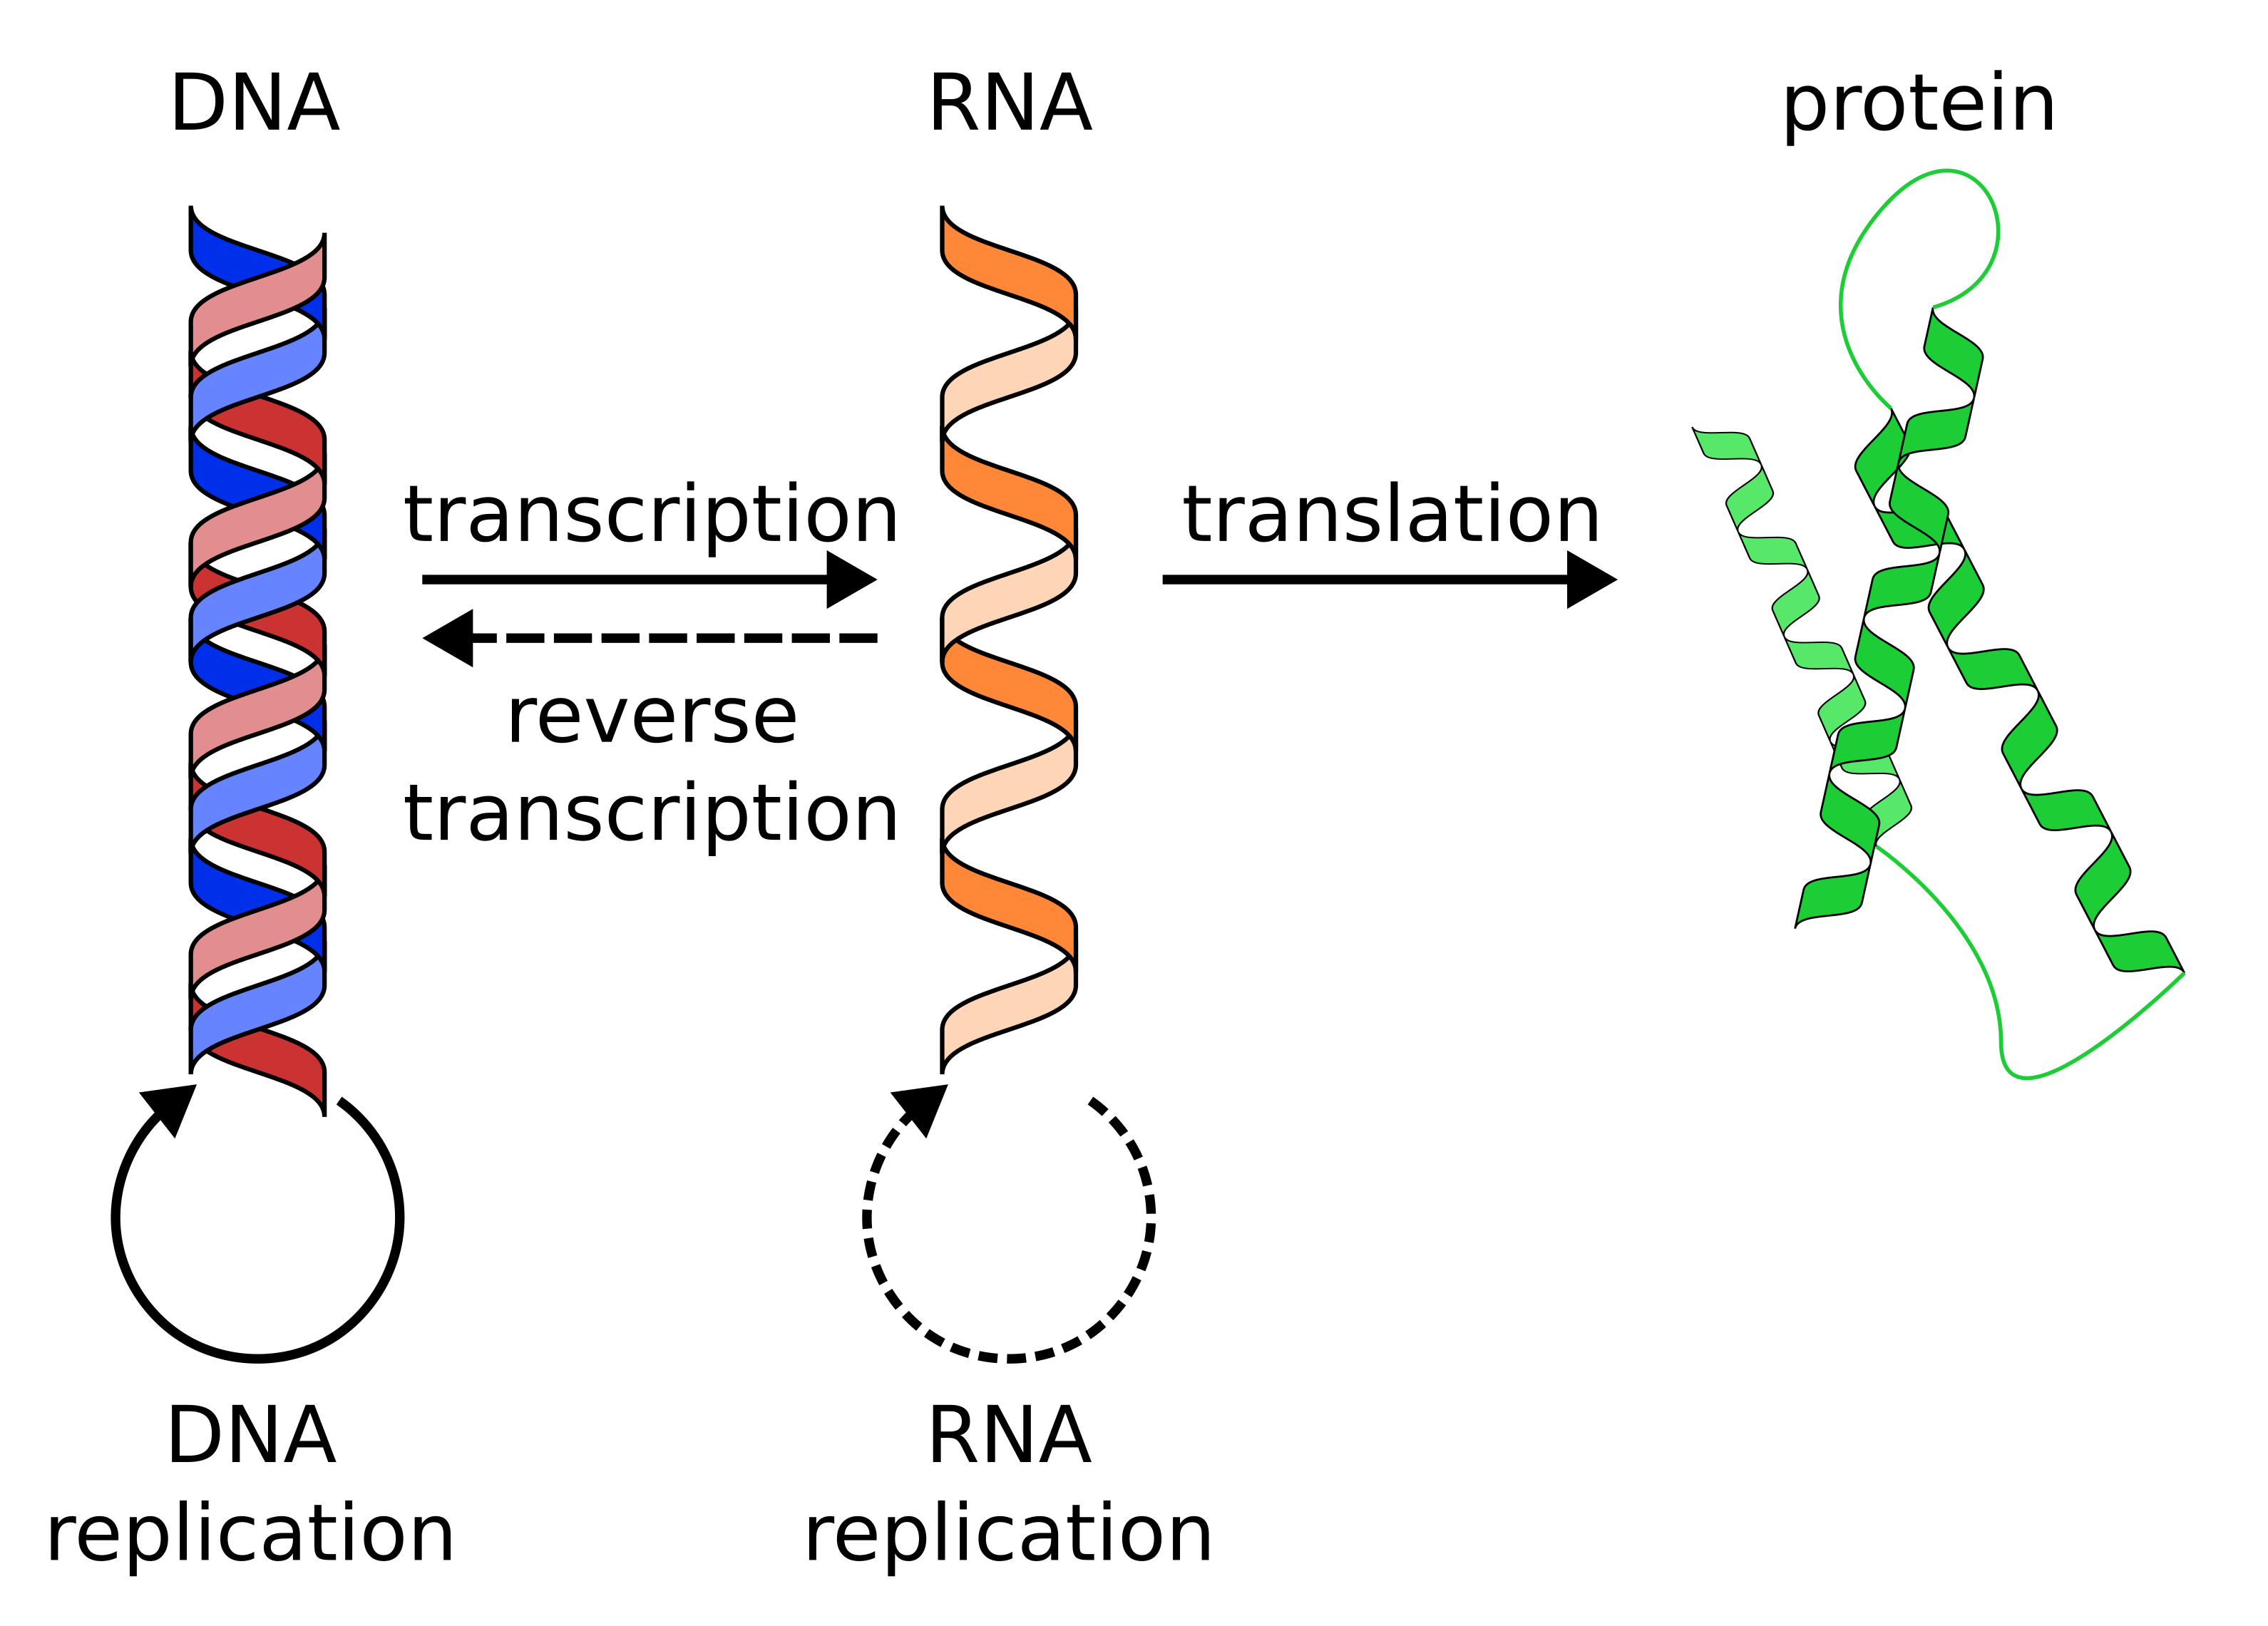
\includegraphics[width=\linewidth]{ch1.Introduction/imgs/central_dogma.png}
    \caption{Caption}
    \label{fig:central_dogma}
\end{figure}

\subsection{Transcription}

\begin{figure}[hbtp]
    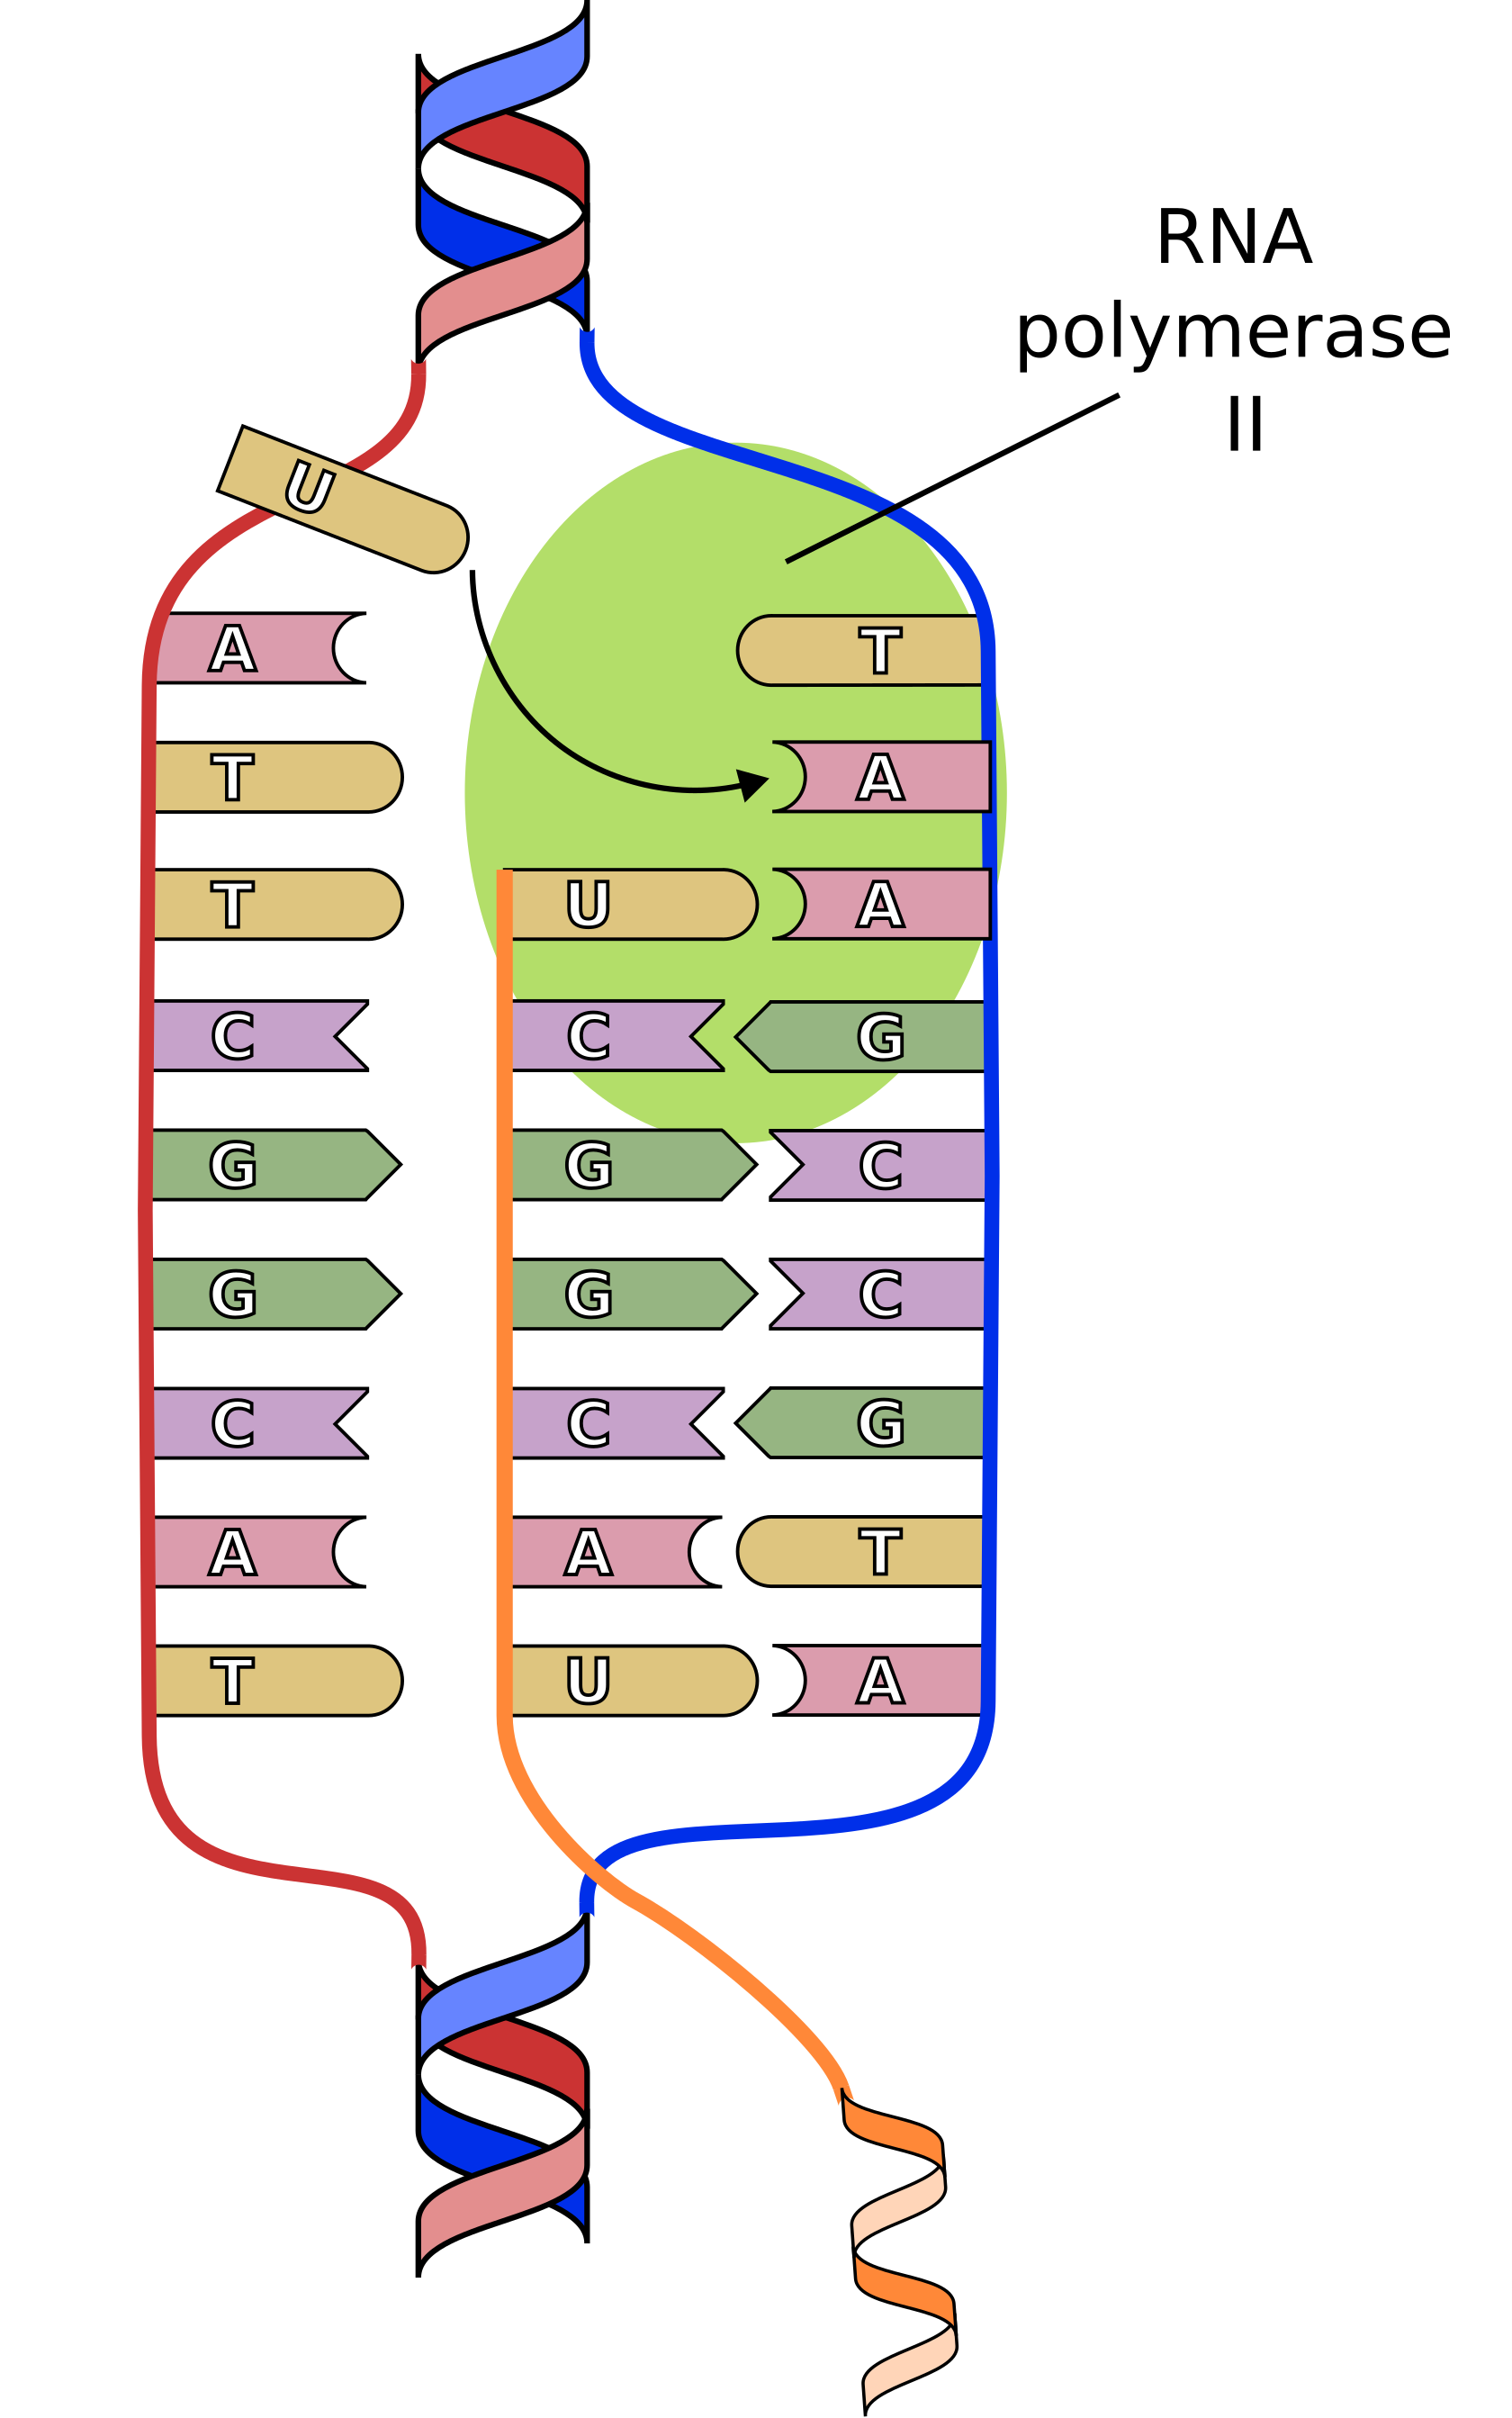
\includegraphics[height=0.9\textheight]{ch1.Introduction/imgs/transcription.png}
    \caption{Caption}
    \label{fig:transcription}
\end{figure}

\subsection{Translation}

\begin{figure}[H]
    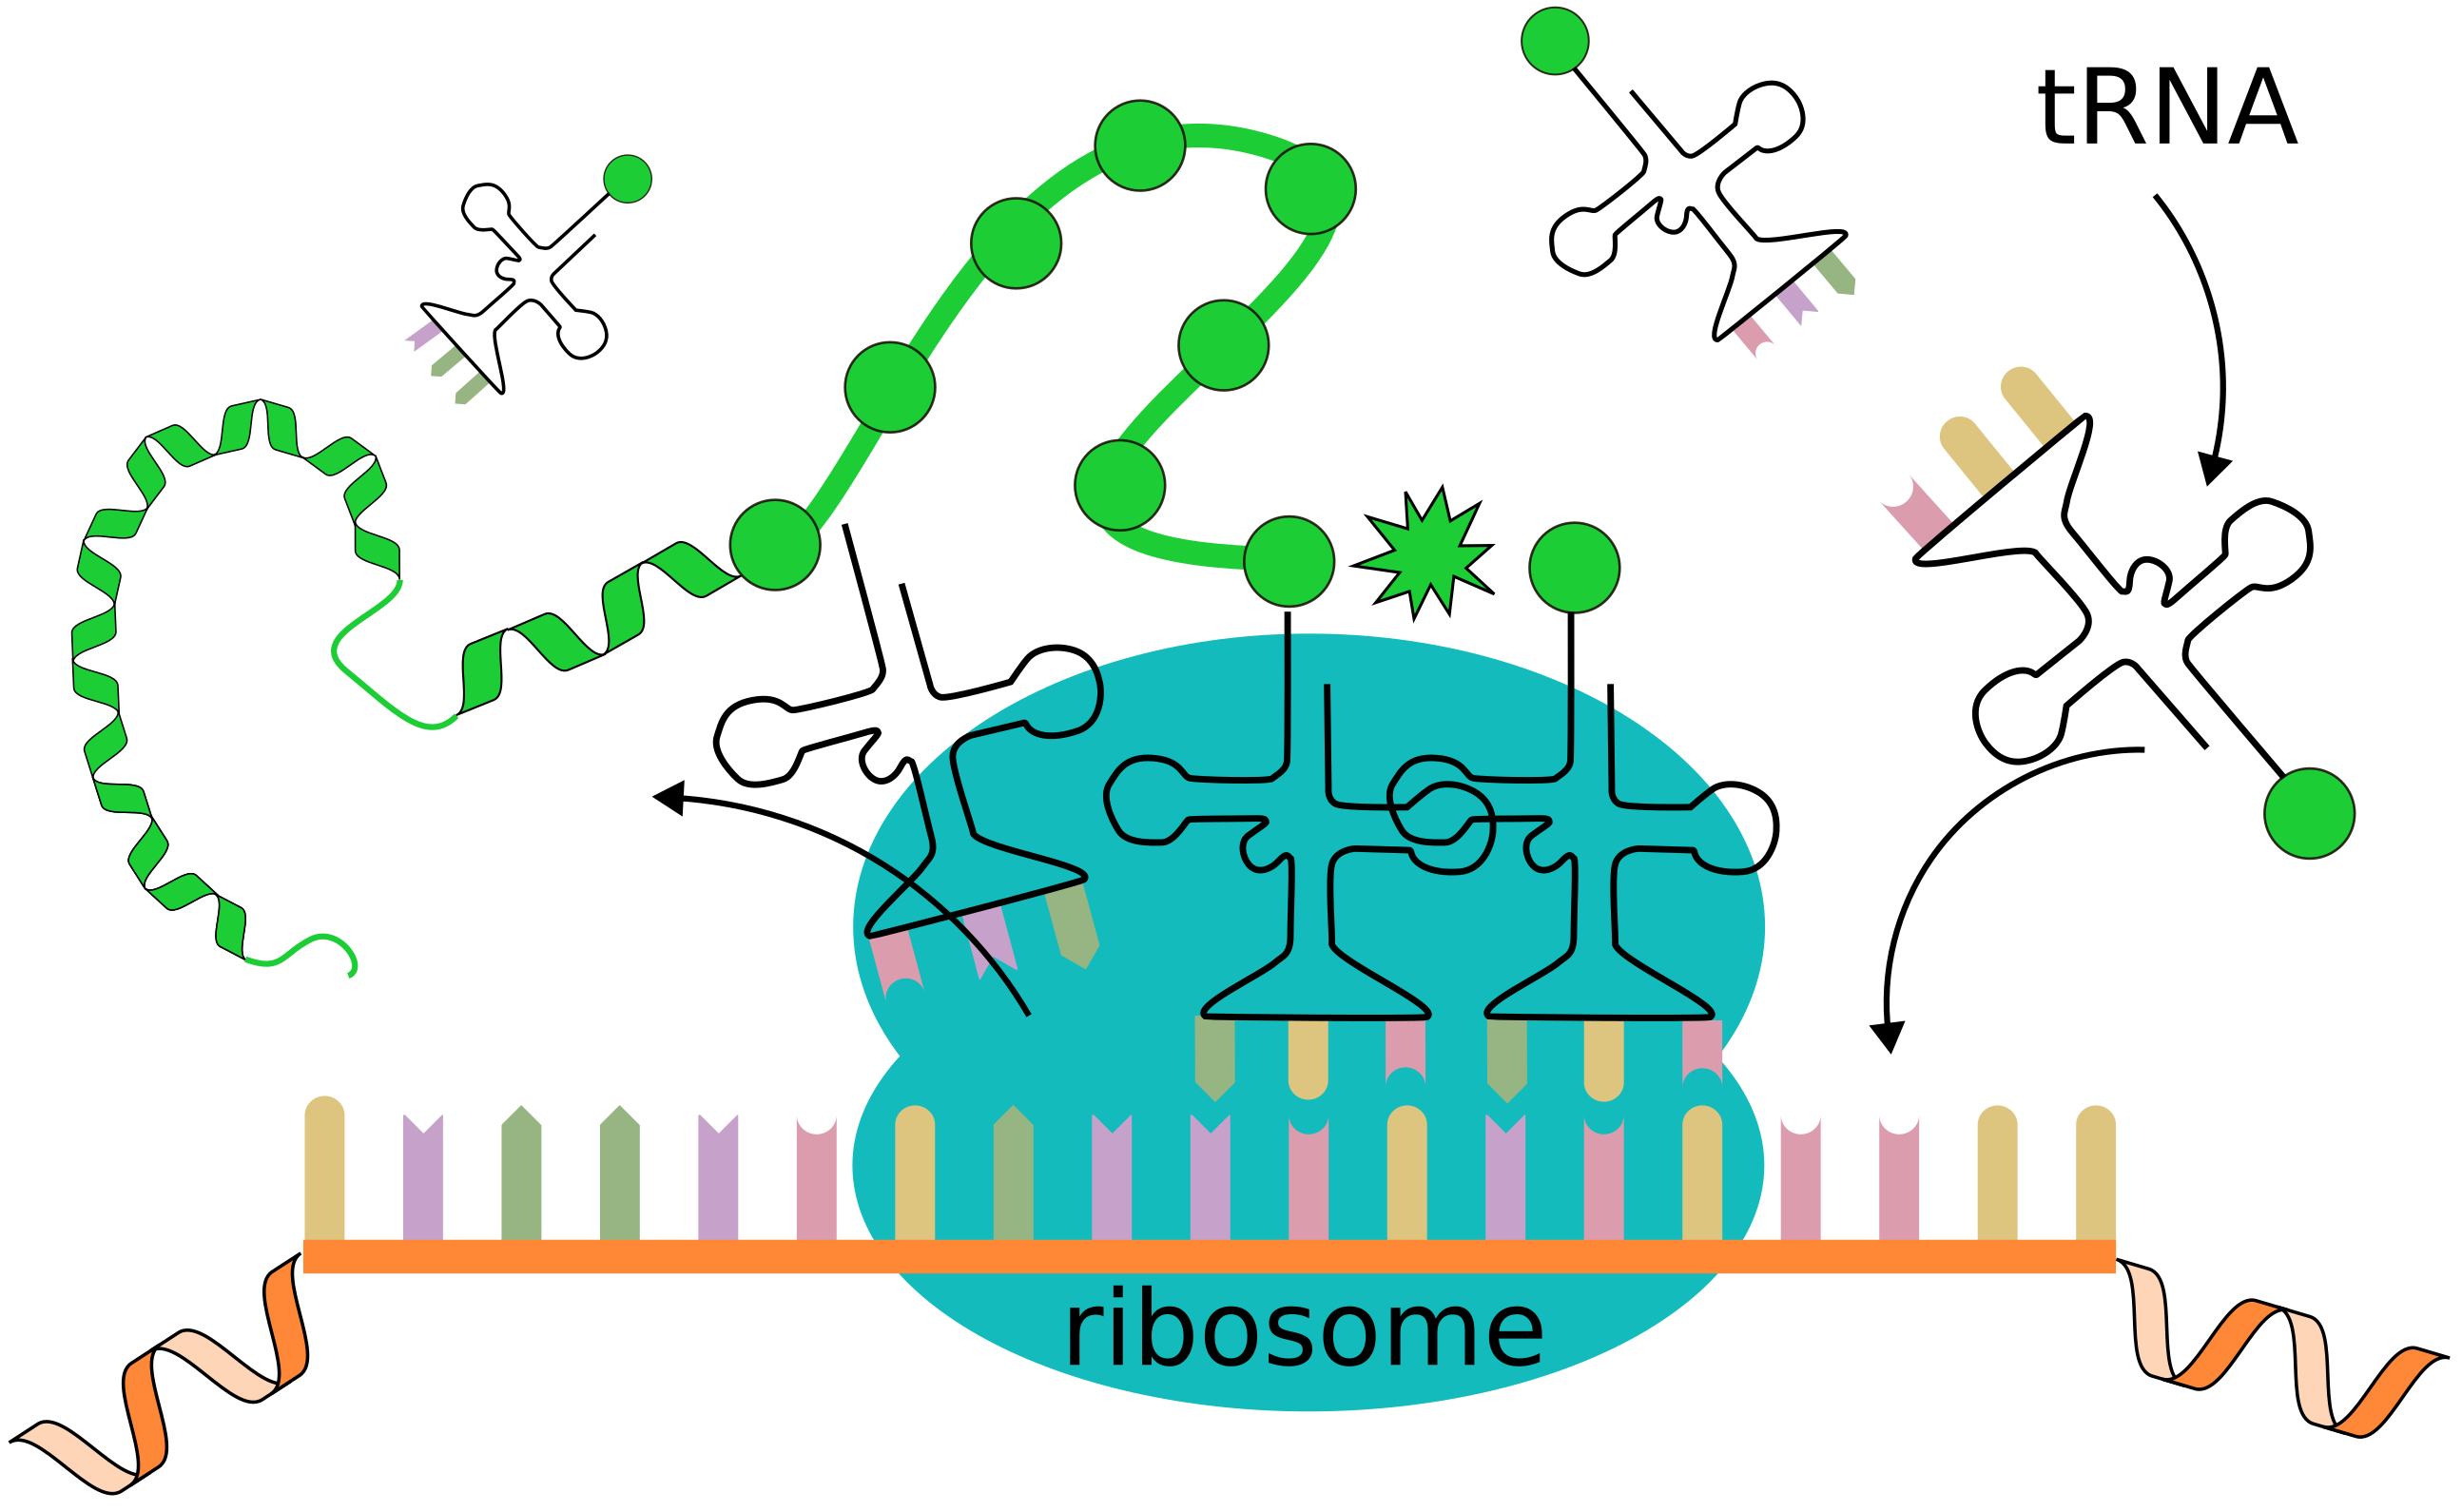
\includegraphics[width=\linewidth]{ch1.Introduction/imgs/translation.png}
    \caption{Caption}
    \label{fig:translation}
\end{figure}

\subsection{Chromatin}

\begin{figure}[H]
    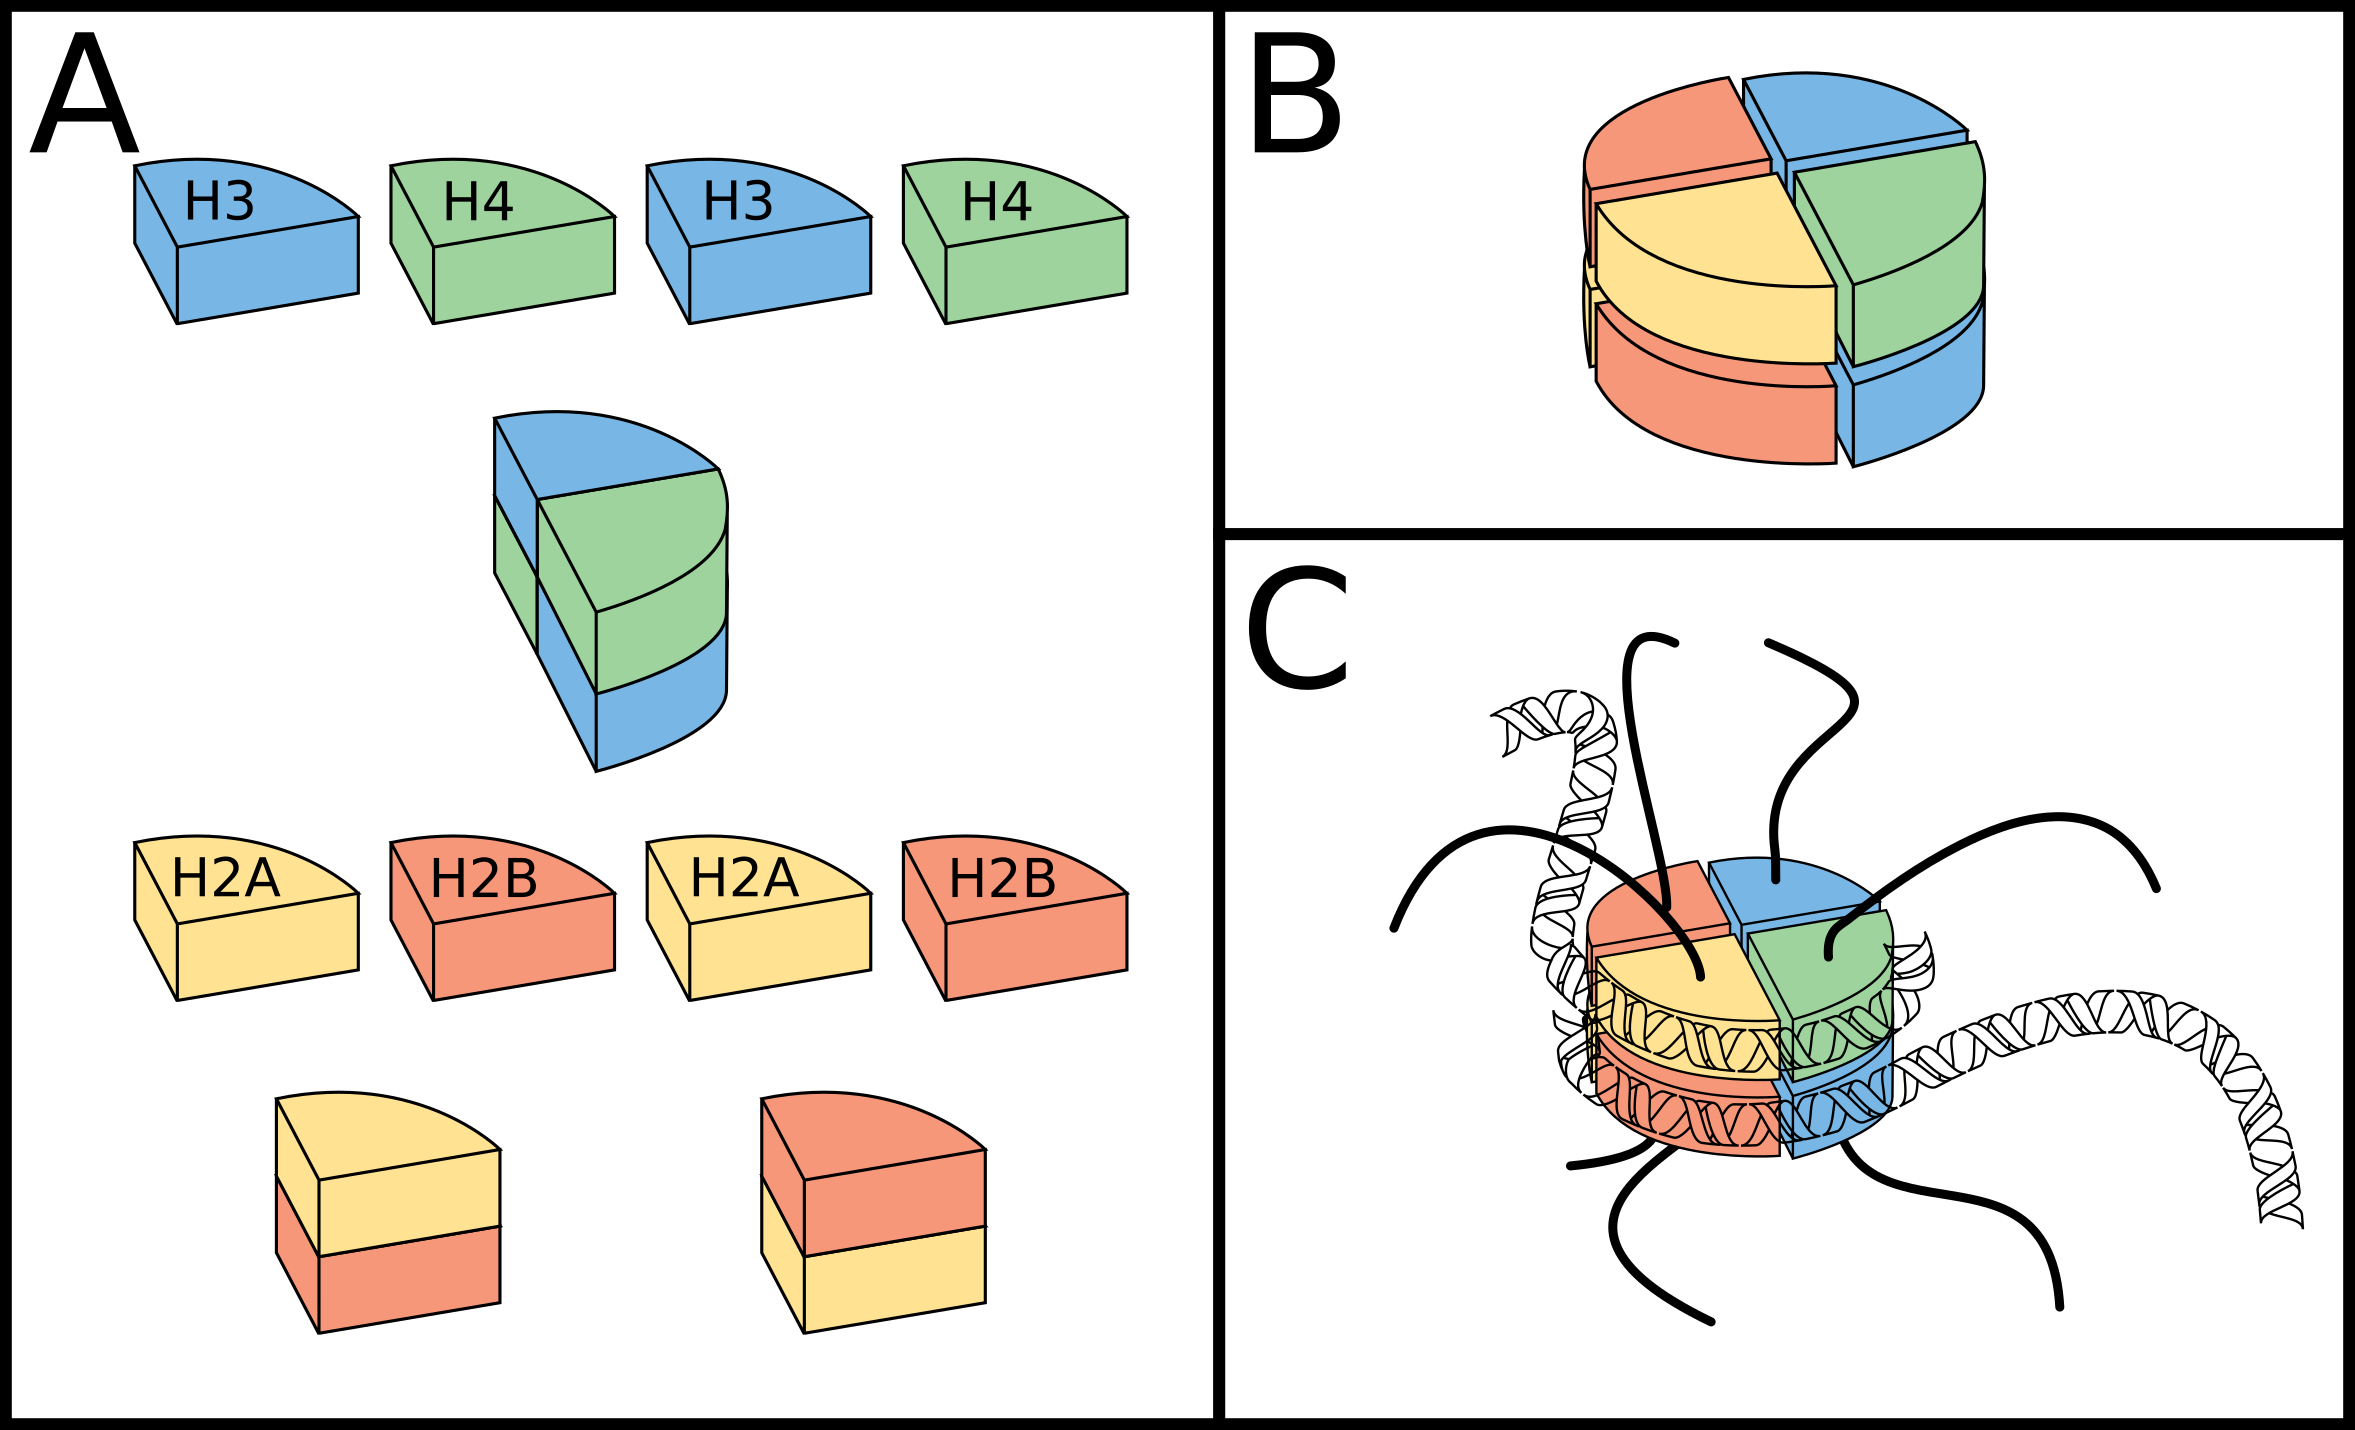
\includegraphics[width=\linewidth]{ch1.Introduction/imgs/histones.png}
    \caption{Caption}
    \label{fig:histones}
\end{figure}

\begin{figure}[hbtp]
    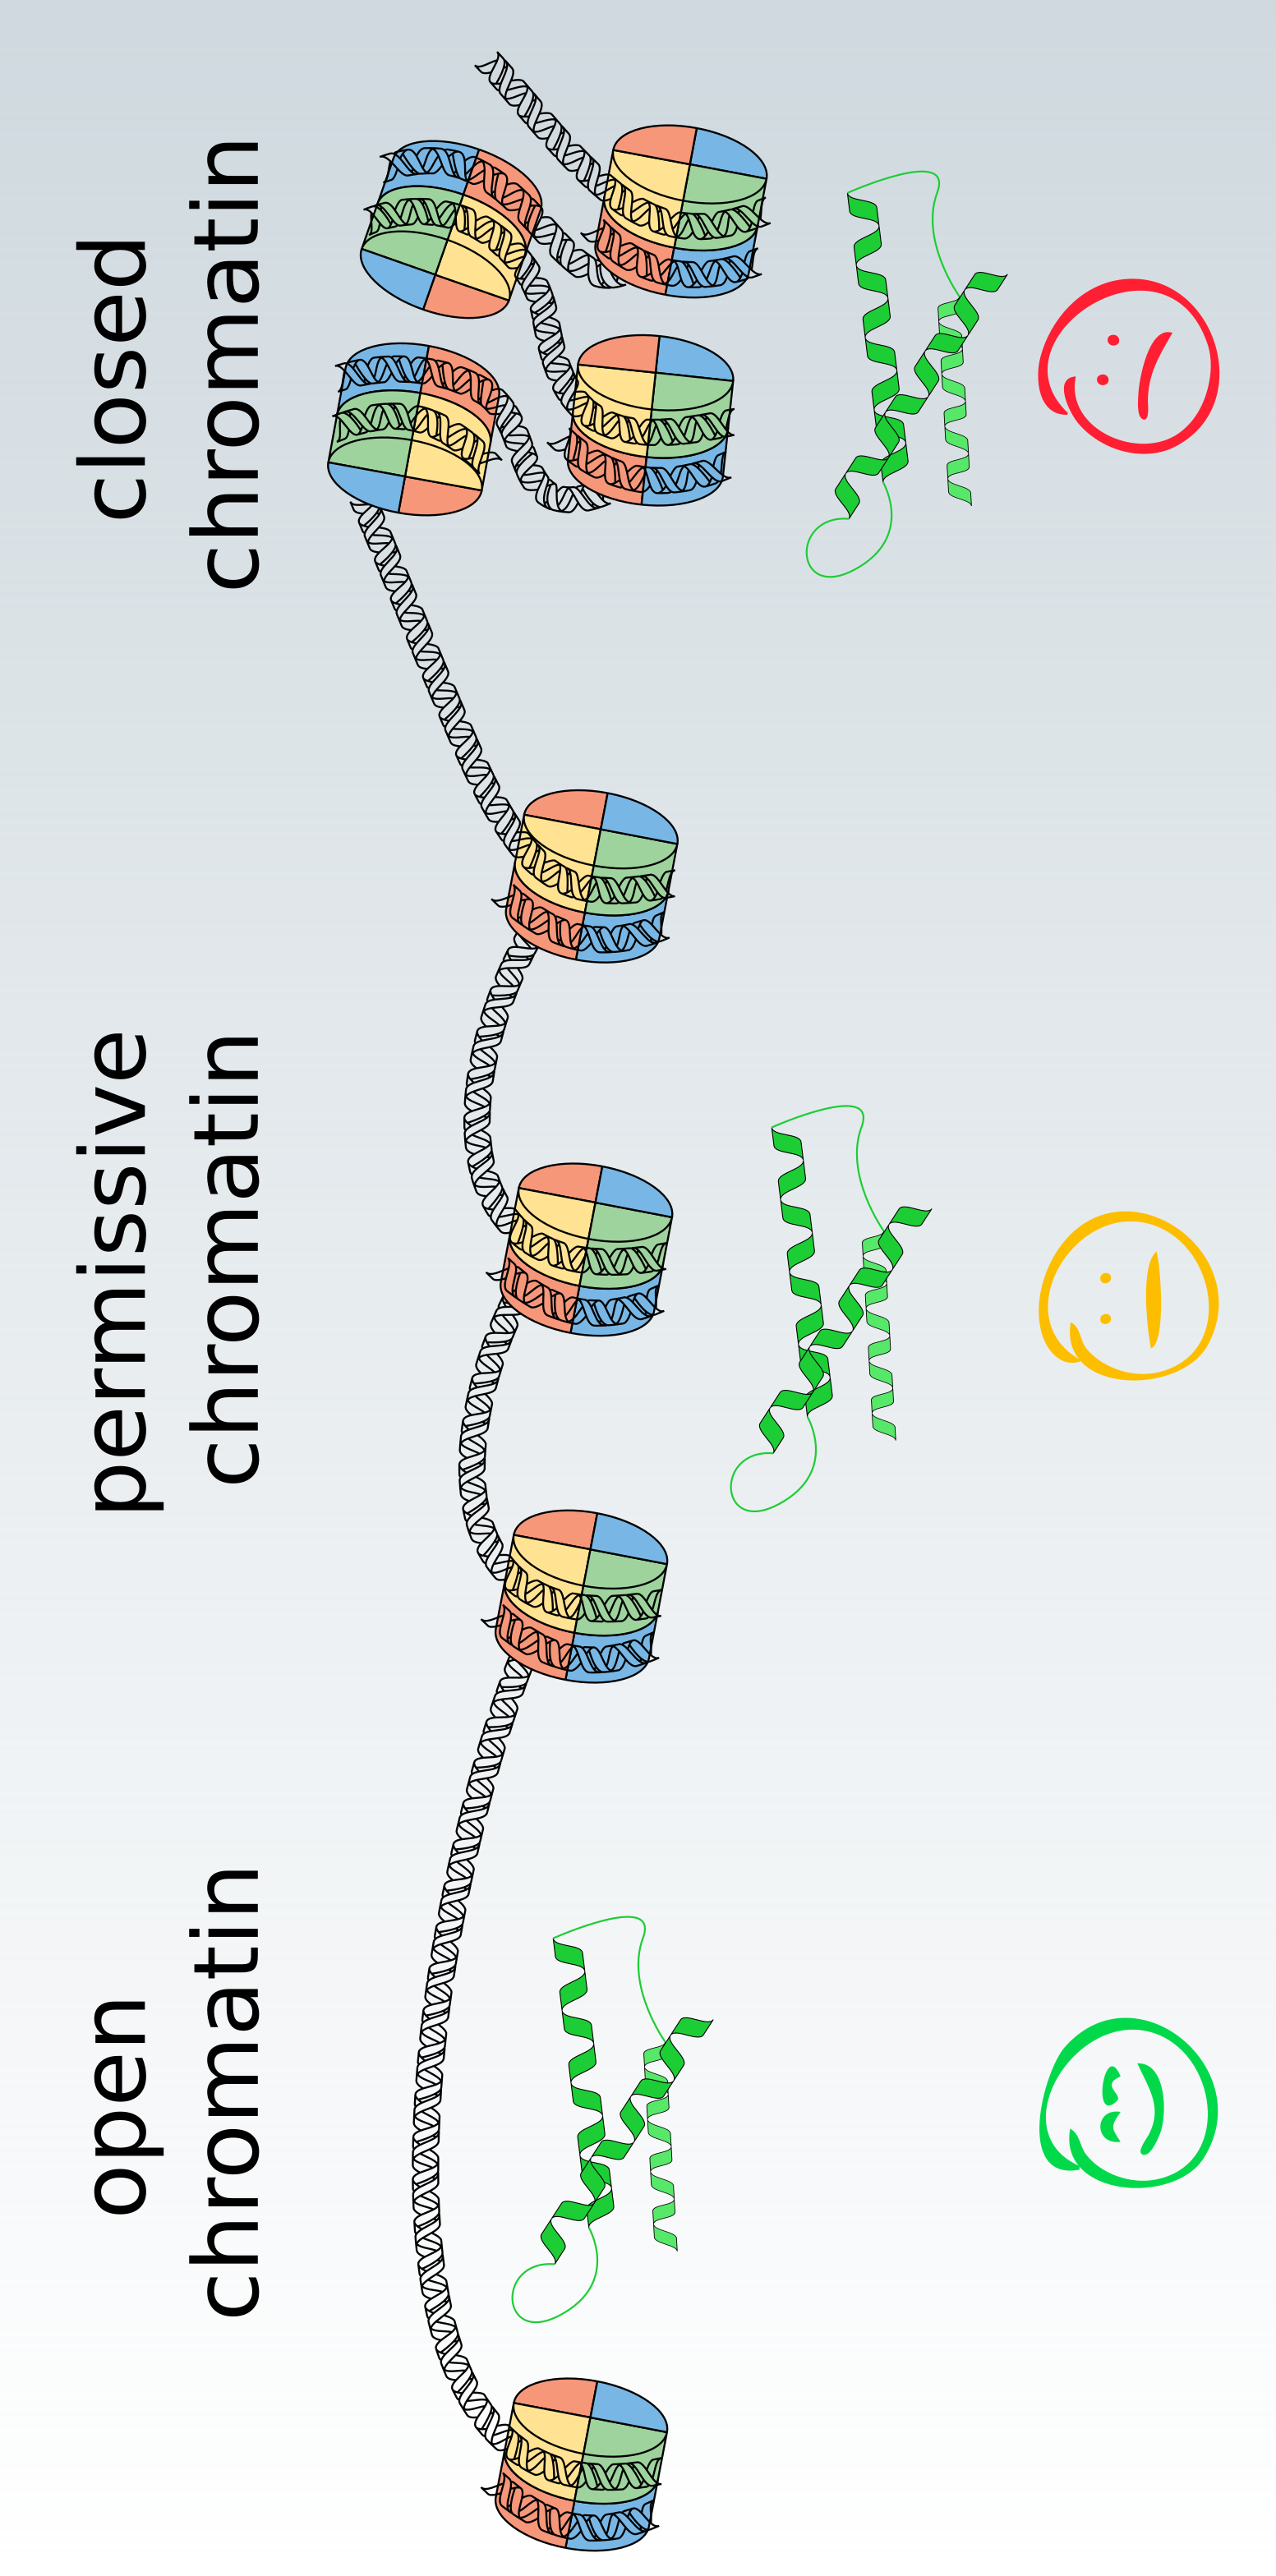
\includegraphics[height=0.9\textheight]{ch1.Introduction/imgs/accessibility.png}
    \caption{Caption}
    \label{fig:accessibility}
\end{figure}

\subsection{Transcription Factors}


\subsection{other regulatory modes}
% \subsubsection{mRNA degradation}
% \subsubsection{Post-transcriptional modification}
% \subsubsection{RNA transport}
% \subsubsection{Signal transduction}
\section{Gene regulatory networks}

\begin{figure}[H]
    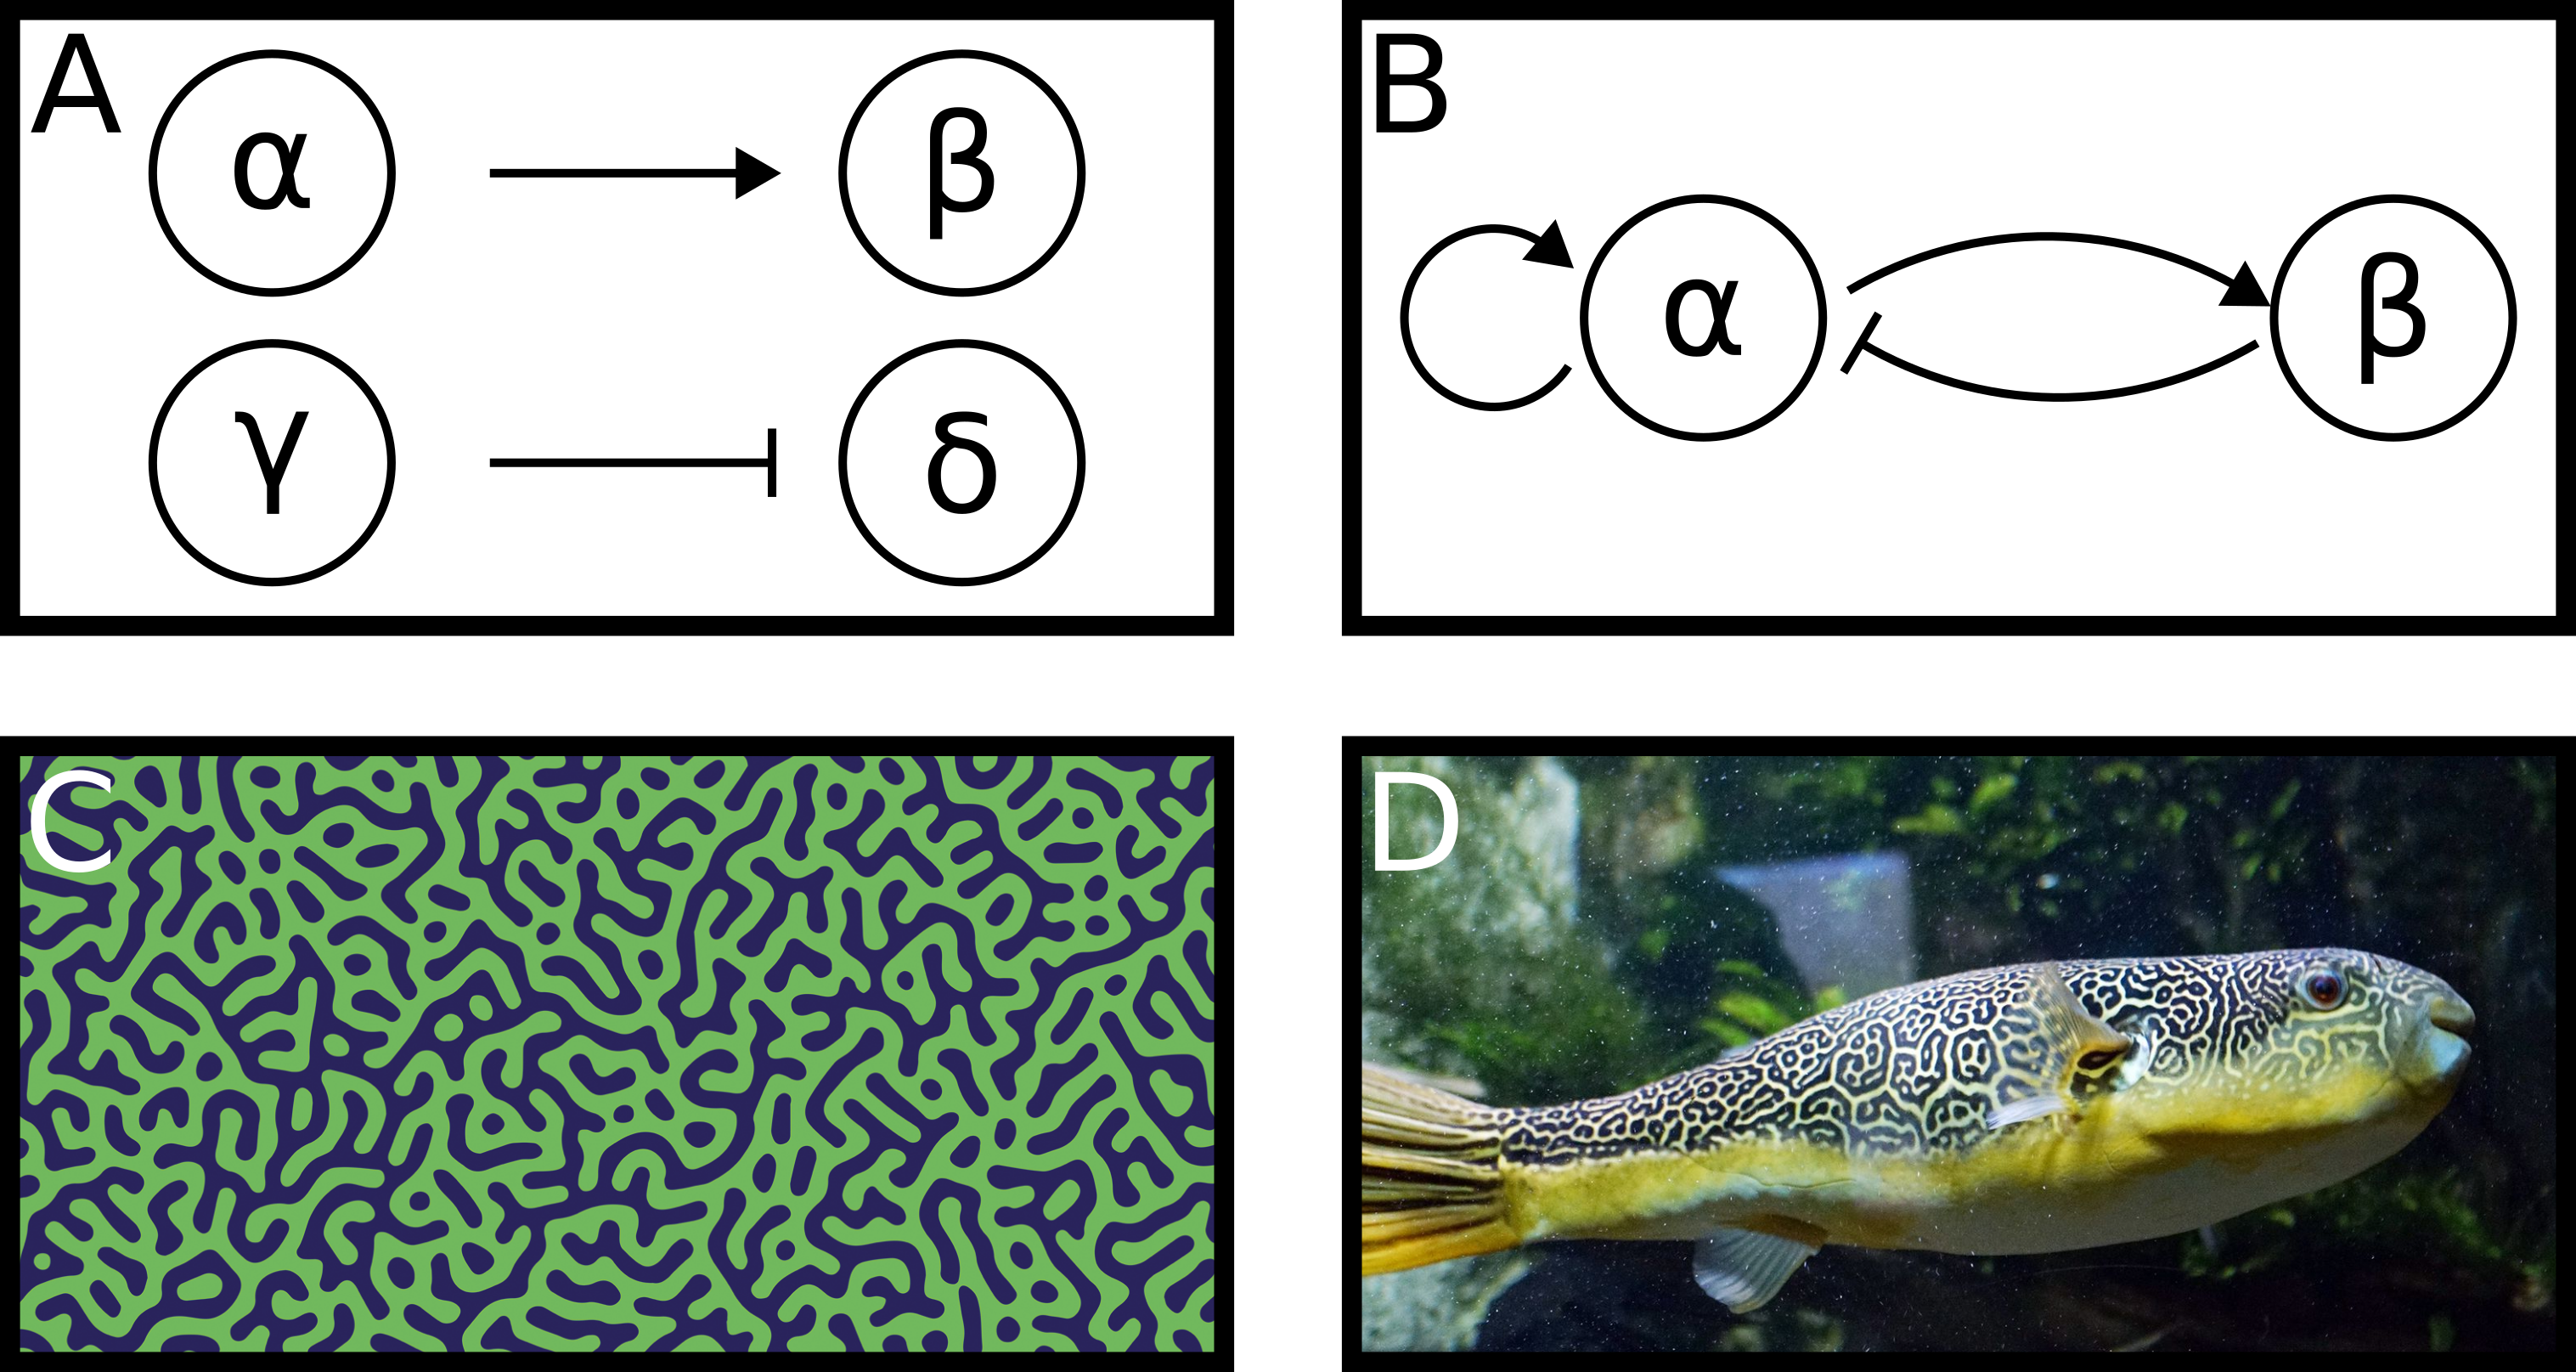
\includegraphics[width=\linewidth]{ch1.Introduction/imgs/network.png}
    \caption{https://en.wikipedia.org/wiki/Mbu\_pufferfish\#/media/File:Tetraodon\_mbu\_2.jpg}
    \label{fig:network}
\end{figure}

\section{Evolution}

\begin{figure}[H]
    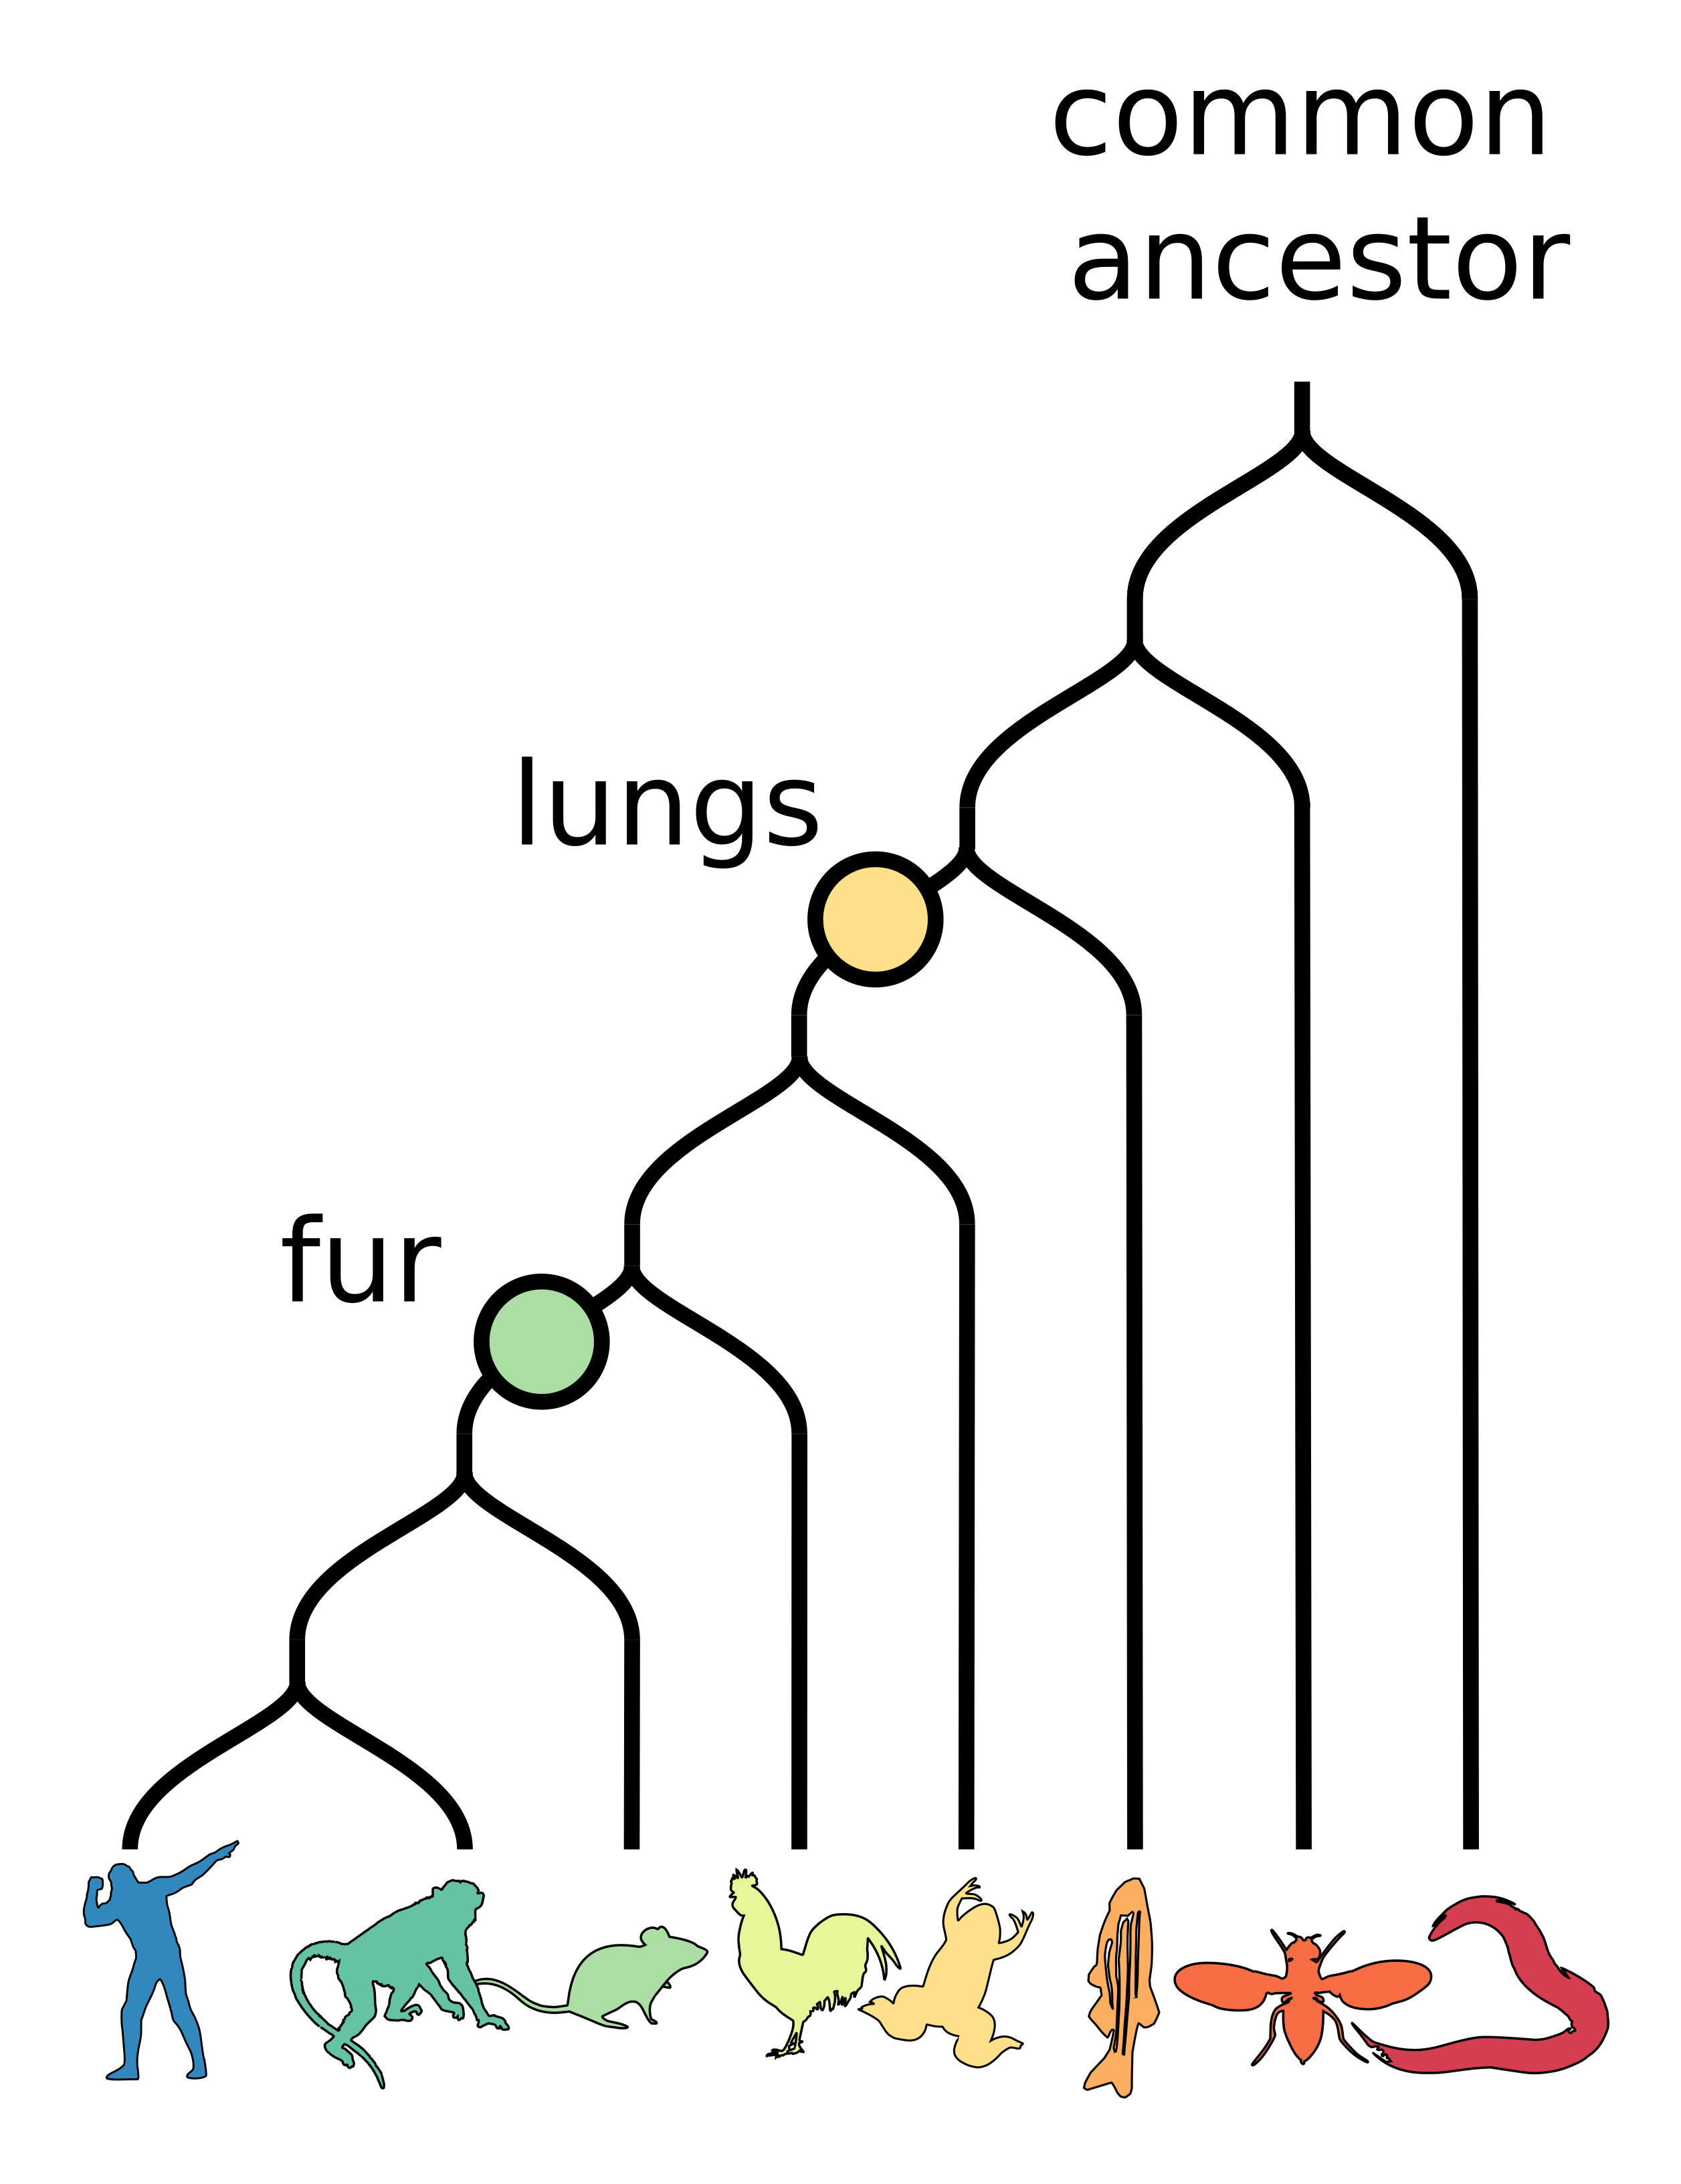
\includegraphics[width=0.5\linewidth]{ch1.Introduction/imgs/phylogeny.png}
    \caption{caption}
    \label{fig:phylogeny}
\end{figure}

\section{Development}

\section{Evolutionary development (evo-devo)}



\subsection{evo-devo gene toolkit}
\subsection{The hourglass model and the phylotypic stage}

\begin{figure}[H]
    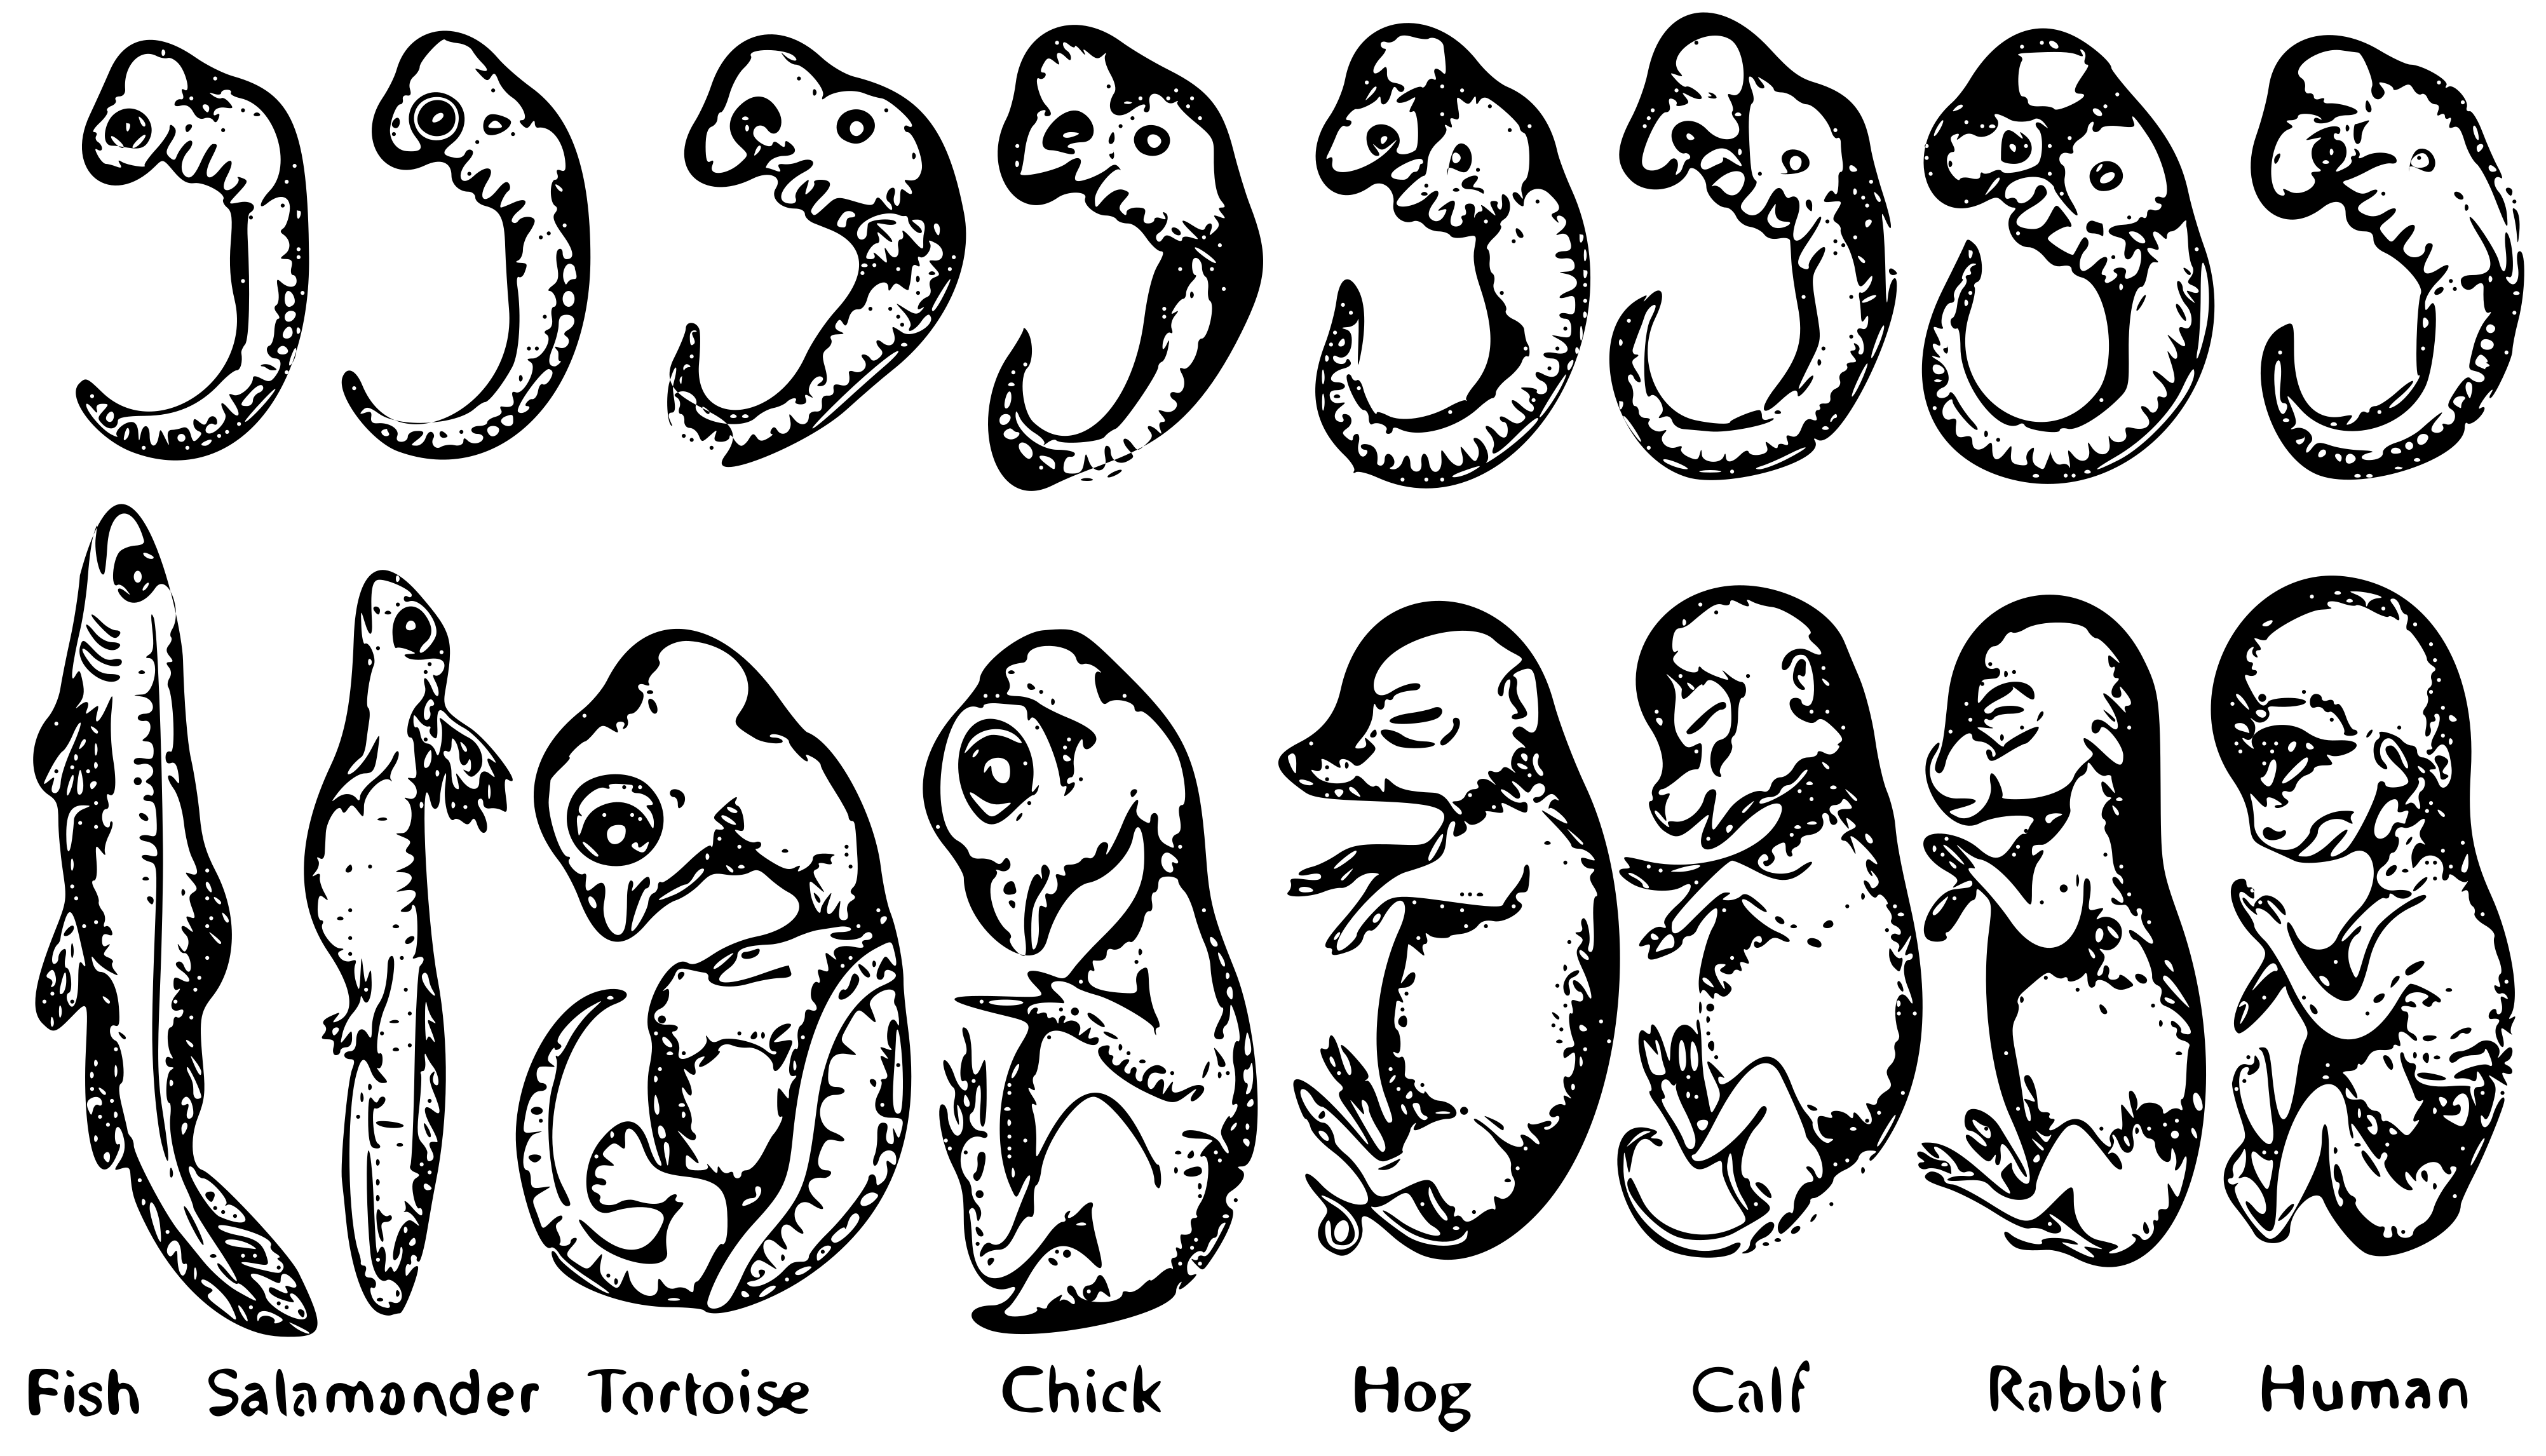
\includegraphics[width=\linewidth]{ch1.Introduction/imgs/haeckel.png}
    \caption{caption}
    \label{fig:haeckel}
\end{figure}

\section{(Computational) genomic analyses}

\begin{figure}[H]
    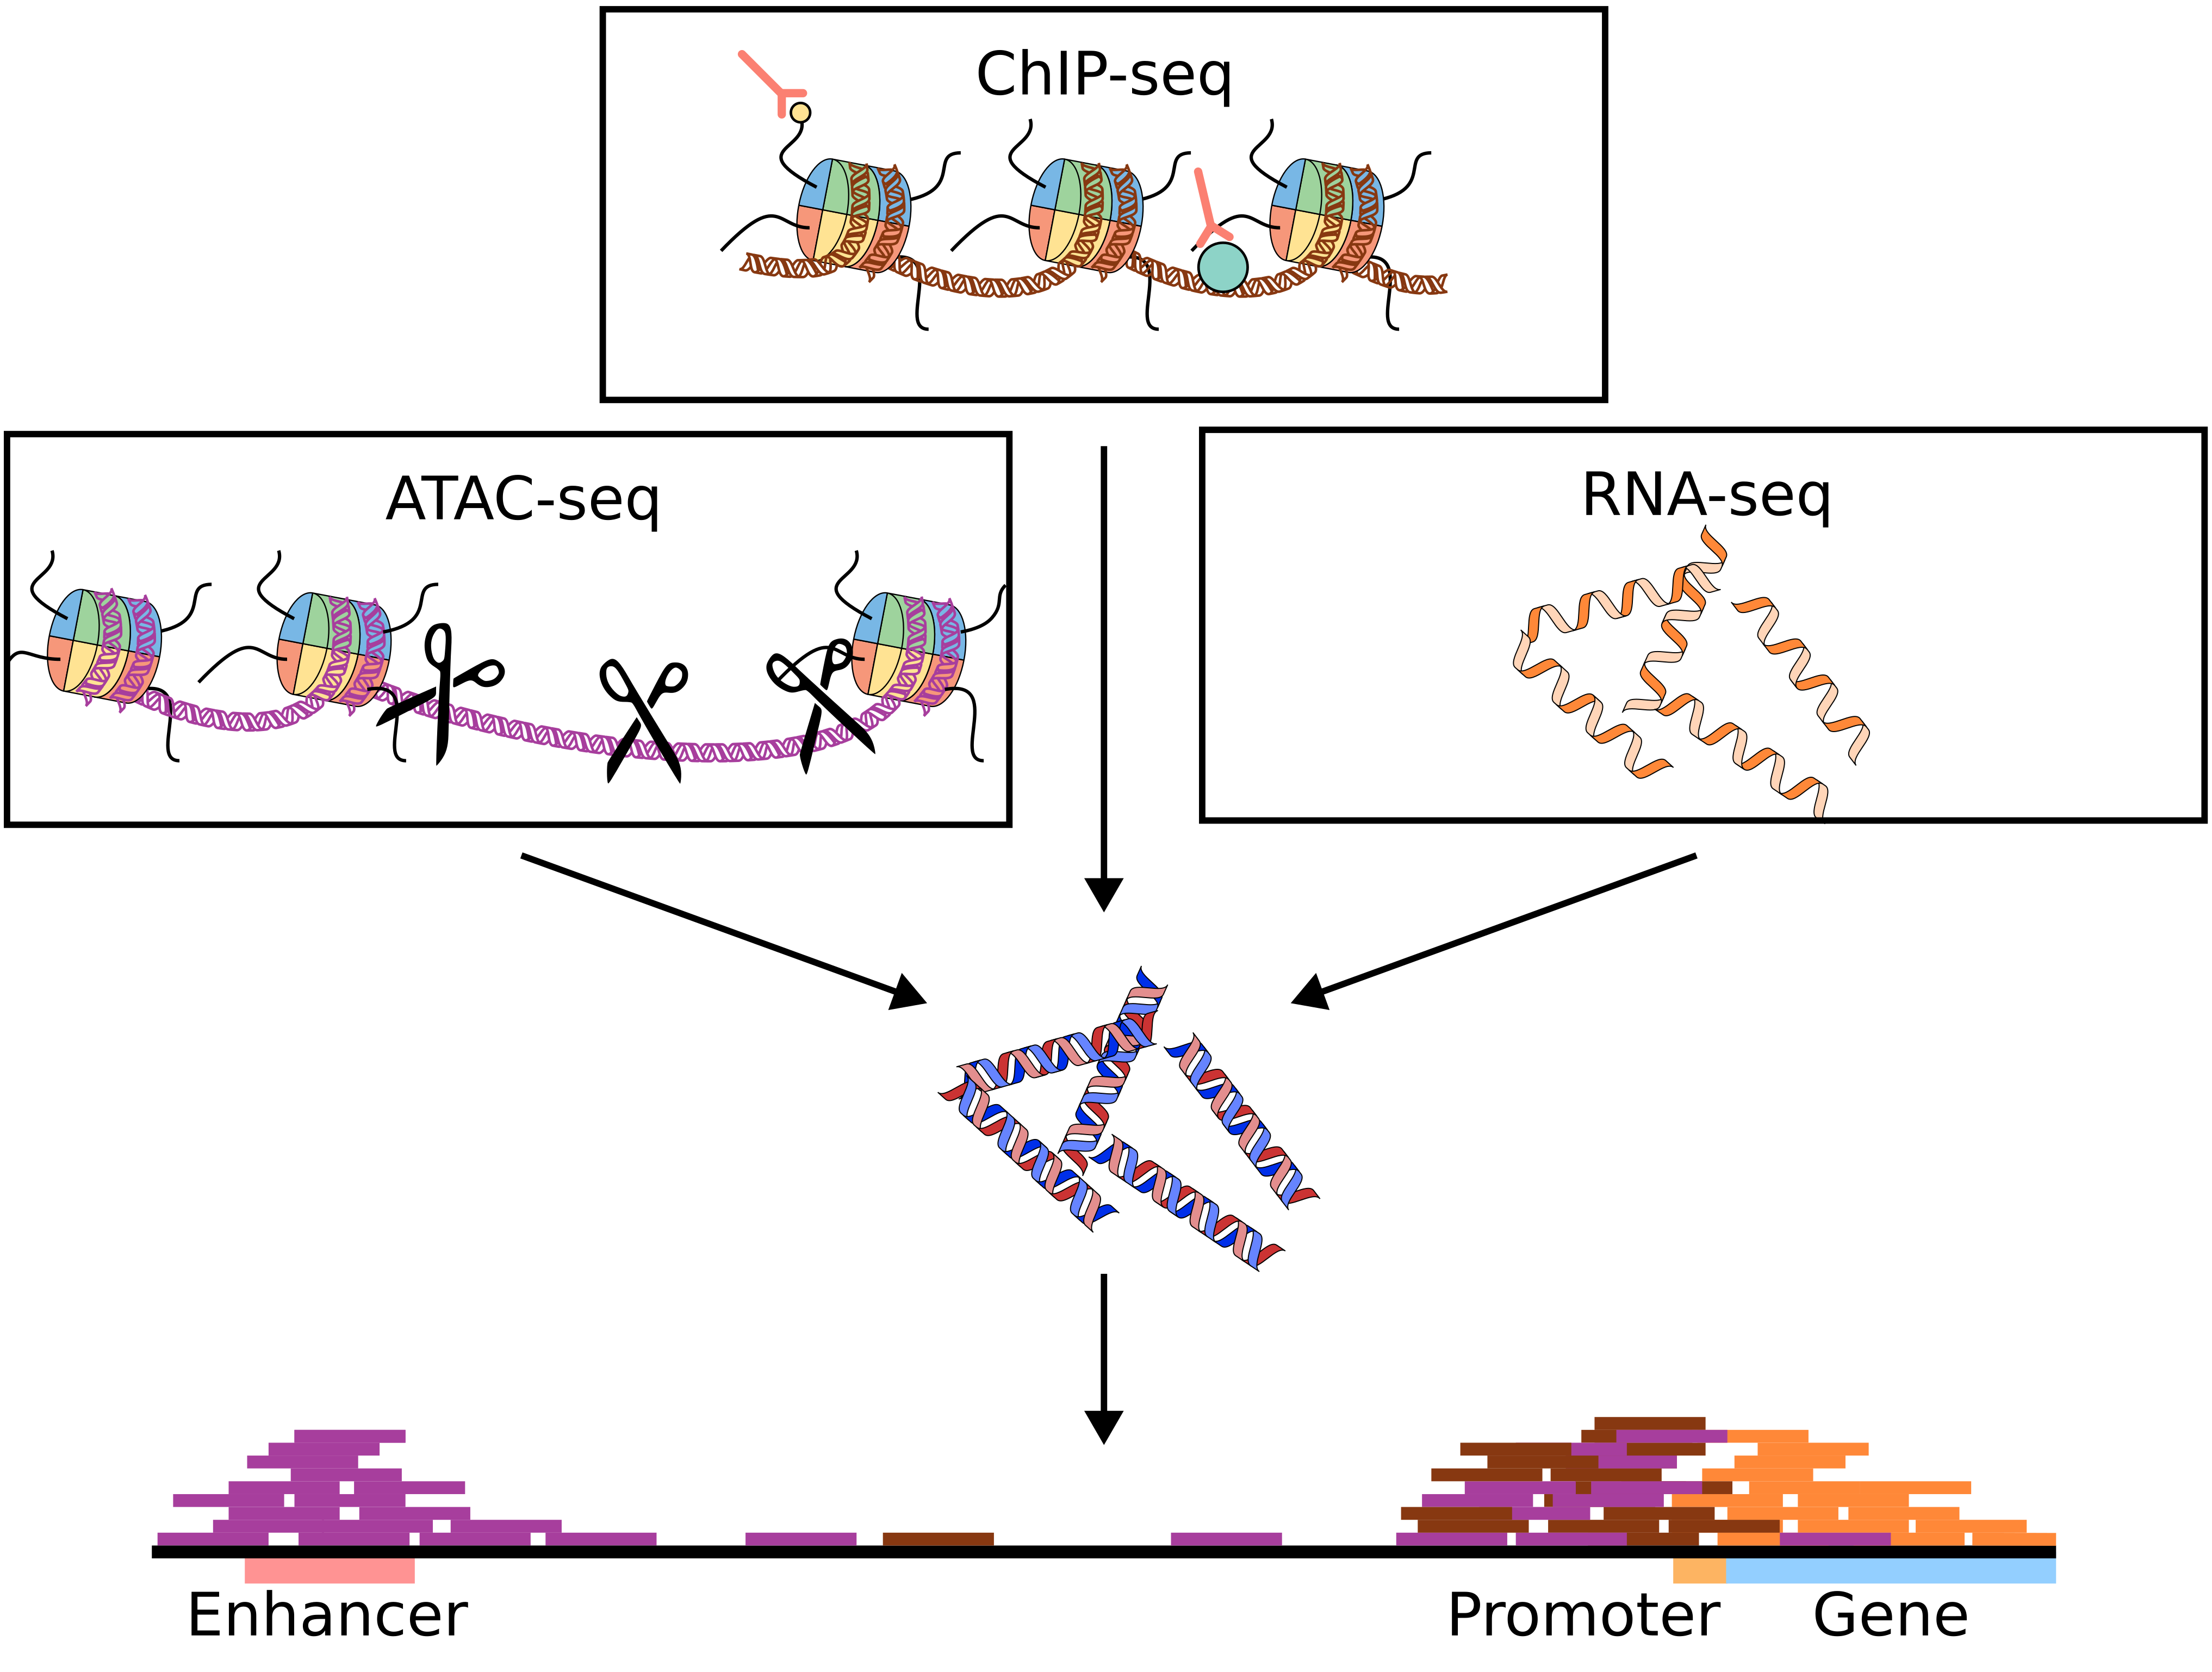
\includegraphics[width=\linewidth]{ch1.Introduction/imgs/analysis.png}
    \caption{caption}
    \label{fig:analysis}
\end{figure}

\subsection{Single cell}

\section{Thesis overview}
